\documentclass[18pt,a4paper]{article}
\usepackage[utf8]{inputenc}
\usepackage{amsmath}
\usepackage{amsfonts}
\usepackage{amssymb}
\usepackage{listings}
\usepackage{color}
\usepackage{textcomp}
\definecolor{listinggray}{gray}{0.9}
\definecolor{lbcolor}{rgb}{0.9,0.9,0.9}
\usepackage{tikz}
\usetikzlibrary{automata,positioning}
\newcommand*\circled[1]{\tikz[baseline=(char.base)]{
            \node[shape=circle,draw,inner sep=1pt] (char) {#1};}}
%\author{kyriakosschwarz}
\title{Einfuehrung in die Theoretische Informatik}



%Math
\usepackage{amsmath}
\usepackage{amsfonts}
\usepackage{amssymb}
\usepackage{amsthm}
\usepackage{ulem}

%PageStyle
%\usepackage[ngerman]{babel} % deutsche Silbentrennung
\usepackage[utf8]{inputenc} 
\usepackage{fancyhdr, graphicx}
\usepackage[scaled=0.92]{helvet}
\usepackage{parskip}
\usepackage[a4paper,top=2cm]{geometry}
\setlength{\textwidth}{17cm}
\setlength{\oddsidemargin}{-0.5cm}


% Shortcommands
\newcommand{\Bold}[1]{\textbf{#1}} %Boldface
\newcommand{\Kursiv}[1]{\textit{#1}} %Italic
\newcommand{\T}[1]{\text{#1}} %Textmode
\newcommand{\Nicht}[1]{\T{\sout{$ #1 $}}} %Streicht Shit durch

%Arrows
\newcommand{\lra}{\leftrightarrow} 
\newcommand{\ra}{\rightarrow}
\newcommand{\la}{\leftarrow}
\newcommand{\lral}{\longleftrightarrow}
\newcommand{\ral}{\longrightarrow}
\newcommand{\lal}{\longleftarrow}
\newcommand{\Lra}{\Leftrightarrow}
\newcommand{\Ra}{\Rightarrow}
\newcommand{\La}{\Leftarrow}
\newcommand{\Lral}{\Longleftrightarrow}
\newcommand{\Ral}{\Longrightarrow}
\newcommand{\Lal}{\Longleftarrow}

%Mine(new)
\newcommand{\tab}{\hspace*{2em}}
\newcommand{\cmark}{\ding{51}}%
\newcommand{\xmark}{\ding{55}}%

\usepackage{amssymb}% http://ctan.org/pkg/amssymb
\usepackage{pifont}% http://ctan.org/pkg/pifont

%Metadata
%\fancyfoot[C]{If you use this documentation for a exam, you should offer a beer to the authors!}
\title{
	\vspace{5cm}
	Einfuehrung in die Theoretische Informatik \\
}
%\author{Kyriakos Schwarz}
\date{HS 2014}





\begin{document}

% Titelbild
\maketitle
\thispagestyle{fancy}
\newpage

% Inhaltsverzeichnis
%\pagenumbering{Roman}
\tableofcontents	  	
\newpage

%\setcounter{page}{1}
\pagenumbering{arabic}

% Inhalt Start

\section{Erste Woche}


\subsection{Sprachen}

Alphabet $\Sigma$: nichtleere endliche \uline{Menge} (von Zeichen)\\
\\
Wort ueber $\Sigma$: endliche \uline{Folge} von Zeichen aus $\Sigma$\\
\\
Leeres Wort: $\epsilon$ (epsilon)\\
\\
Menge aller Woerter ueber $\Sigma$: $\Sigma^*$\\
\\
\\
Konkatenation von Woertern $x,y$ ueber $\Sigma$:\\
\\
$x = x_1x_2 ... x_n$ \tab ,$x_i \in \Sigma$\\
$y = y_1y_2 ... y_n$\tab\:\: ,$y_i \in \Sigma$\\
\\
$x \cdot y = xy = x_1x_2 ... x_ny_1y_2 ... y_n$\\
\\
Java: $+$\tab\tab $""$ ($\epsilon$)\\
Haskell: $++$\tab $""$ ($\epsilon$)\\
\\
\\
\uline{Monoid}: Sei $M$ eine Menge und\\
\tab $\circ : M \times M \rightarrow^{total} M$ eine Verknuepfung\\
\\
Das Paar $(M, \circ)$ heisst ein \uline{Monoid}, falls gilt:\\
\\
1) $a \circ (b \circ c) = (a \circ b) \circ c$\tab ,$\forall a,b,c \in M$\\
\\
2) Es gibt ein $e \in M$ mit $a \circ e = a = e \circ a$\tab ,$\forall a \in M$\\
\\
$\qed$\\
\\
\\
\uline{Beispiel 1}\\
\\
$M = \Sigma^*, \circ = \cdot$\\
\\
$(\Sigma^*, \cdot)$ ist ein Monoid mit $\epsilon$ als neutralem Element\\
\\
$\qed$\\
\\
\uline{Beispiel 2}\\
\\
$\{\{ x =5; y = 6;\} z =7;\} \equiv \{x =5; \{y =6; z=7;\}\}$\\
\\
Komposition von Anweisungen assoziativ\\
\\
Neutrales Element: $;$ (Java) skip, NOP (no operation)\\
\\
$(x = 2*x; x = x+1;) \not\equiv (x = x+1; x = 2*x)$\\
\\
$\qed$\\
\\
\\
\uline{Sprache ueber $\Sigma$}:\\
\\
Menge von Woerter ueber $\Sigma$\\
\\
\uline{Beispiele}\\
\\
$\{\}$\tab 0 Woerter\\
$\{0,1,01,10\}$ Sprache uber $\Sigma = \{0,1\}$\\
$\Sigma^*$\\
$\{\epsilon\}$\tab 1 Wort\\
$\{\epsilon, 0, 00, 000, ...\}$ uber $\Sigma = \{0\}$\\
\\
\uline{Bem}\\
Sprache kann $\infty$ viele Woerter enthalten\\
Jedes Wort ist aber endlich\\
\\
\uline{Bem}\\
$\epsilon \in \Sigma^*$\\
$\Sigma^*$ immer $\infty$ gross\\
\\
\\
\uline{Operationen auf Sprachen}\\
\\
Seien $L_1$, $L_2$ Sprachen\\
\\
$L_1\cup L_2$ Vereinigungsmenge\\
\\
$L_1 \cdot L_2 = \{ xy \:\vert\: x \in L_1, y \in L_2\}$ (Kreuzprodukt)\\
\\
\\
Sei $(M, \circ)$ ein Monoid. Dann def.\\
\\
$a^0 = e$\tab\tab\:\:\:  ,$a \in M$\\
$a^n = a \circ a^{n-1}$\tab ,$n > 0$\\
\\
$\qed$\\
\\
\\
$L^0 = \{\epsilon\}$\\
\\
$L^n = L \cdot L^{n-1}$\tab ,$n>0$\\
\\
\\
\uline{Kleen' scher Stern}\\
\\
$L^* = L^0 \cup L^1 \cup L^2 \cup ...$\\
\\
\tab $= \{x_1, x_2, ..., x_k \:\vert\: k \geqslant 0, x_i \in L\}$\\
\\
\\
\uline{Aufgabe}\\
\\
$\Sigma = \{a,b,...,z\}$, $L_1 = \{good, bad\}$, $L_2 = \{cat, dog\}$\\
\\
$L_1 \cup L_2 = \{bad, cat, dog, good\}$\\
\\
$L_1 \cdot L_2 = \{goodcat, gooddog, badcat, baddog\}$\\
\\
$L_1^0 = \{\epsilon\}$\\
\\
$L_1^1 = \{good, bad\} = L_1 \cdot L_1^0 = L_1$\\
\\
$L_1^2  = \{goodgood, goodbad, badgood, badbad\}$\\
\\
$L_1^3 = \{ goodgoodgood, goodgoodbad, goodbadgood, goodbadbad,$\\
\tab\:\:\: $badgoodgood, badgoodbad, badbadgood, badbadbad\}$\\
\\
$L_1^* = L_1^0 \cup L_1^1 \cup L_1^2 \cup L_1^3 \cup ...$\\
\tab $= \{x_1, x_2, ..., x_k \:\vert k \geqslant 0, x_i \in, L_1\} = \{\epsilon, ...\}$\\
\\
$L_1 \cdot L_2 = \{goodcat, gooddog, badcat, baddog\} \neq L_2 \cdot L_1$\\
\\
$\vert M \vert =$ Anzahl Elemente von $M$\\ 
\\
\\
\rule{\textwidth}{0.4mm}\\
\subsection{Endliche Automaten DFA}

\uline{d}eterministic \uline{f}inite \uline{a}utomator\\
\\
\uline{Statisch}\\
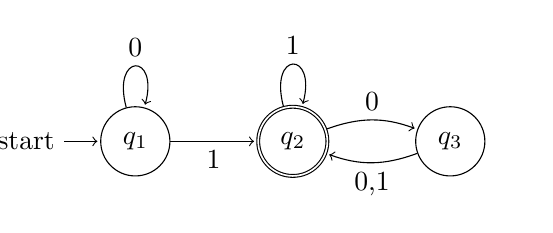
\begin{tikzpicture}[shorten >=1pt,node distance=2cm,on grid,auto] 
   \node[state,initial] (q_1)   {$q_1$}; 
%   \node[state] (q_1) [above right=of q_0] {$q_1$}; 
   \node[state, accepting] (q_2) [right=of q_1] {$q_2$}; 
   \node[state](q_3) [right=of q_2] {$q_3$};
    \path[->] 
%    (q_1) edge  node {0} (q_1)
%          edge  node [swap] {1} (q_2)
    (q_1) edge  node [swap] {1} (q_2)
          edge [loop above] node {0} ()
    (q_2) edge [bend left=20] node {0} (q_3)
          edge [loop above] node {1} ()      
    (q_3) edge [bend left=20] node {0,1} (q_2); 
%          edge [loop below] node {1} ();
\end{tikzpicture}
\\
\\
\uline{Dynamisch}\\
\\
\uline{Verarbeitung}\tab Input: $\xrightarrow{1101}$\\
\\
1. Start in $q_1$\tab Startzustand\\
2. Lese $\circled{1}101$\tab, $q_1 \rightarrow q_2$\\
3. Lese $1\circled{1}01$\tab, $q_2 \rightarrow q_2$\\
4. Lese $11\circled{0}1$\tab, $q_2 \rightarrow q_3$\\
5. Lese $110\circled{1}$\tab, $q_3 \rightarrow q_2$\\
6. Fertig $+$ akzeptiere, da $q_2$ akzeptierender Zustand ist und die Eingabe fertig gelesen ist.\\
\\
Liefert \uline{accept} oder \uline{fertig}\\
\\
\uline{Terminiert immer!}\\
\\
\\
\uline{Def}  \uline{DFA} : Ein DFA ist ein 5-Tupel $(Q, \Sigma, \delta, q_0, F)$ mit:\\
\\
1. $Q$ ist eine endliche nichtleere Menge von Zustaenden\\
\\
2. $\Sigma$ ist das \uline{Eingabealphabet} (z.B. $1101$)\\
\\
3. $\delta : Q \times \Sigma \rightarrow^{total} Q$\\
\tab \uline{Transitionsfunktion}\\
\\
4. $q_0$ Startzustand\\
\\
5. $F \subseteq Q$ Menge der akzeptierende Zustaende\\
\\
\\
\rule{\textwidth}{0.4mm}\\
\\
 


\end{document}